
\section{Specific Requirements}


\subsection{Functional Requirement}

With these requirements are defined features and functions with which
the user will interact directly.



\subsubsection{{[}G1{]} Allow guests to register to "PowerEnJoy'' service through both website or mobile application.}
\begin{itemize}
	\reqcounter The system shall allow registration only if the patent license number is provided.
	\reqcounter The system shall provide a home page in which a guest user must be
	able to know what the service is. 
	\reqcounter The system shall demand the User to read and accept all term of use of the service.
	\todo{[Andrea] New}
	\reqcounter The system shall provide a form in which a Guest can insert his personal data for the registration to the service.
	
	\reqcounter The system shall provide a form in which a Guest can insert his payment information.
	
	
\end{itemize}

\subsubsection{{[}G2{]} Allow registered users to login and logout.}
\begin{itemize}
	\reqcounter The system shall show a sign-up page with a login form and a logout button if the User is already logged in.
	\reqcounter The system shall validate any input in both client and server side.
	\reqcounter The system shall prevent anyone from logging more than once at a time.
	\reqcounter The system shall show and error message in case of wrong credential.
	\reqcounter The system shall provide a password recovery procedure.
	\reqcounter The system shall prevent bruteforce attack limiting the number of try per IP address.
	\reqcounter The system shall redirect the User to the homepage as a guest after the logout.
\end{itemize}



\subsubsection{{[}G3{]} Allow authenticated users to modify their personal details and payment informations.}
\begin{itemize}
	\reqcounter The system shall show a an account page with all the information that the User sent during 
	account registration.
	\reqcounter The system shall ask for the password before saving the edited details.
	\reqcounter The system shall send and email to notify the changes.
\end{itemize}



\subsubsection{{[}G4{]} Allow authenticated users to view a list of available car in a configurable radius of 
	distance from user position or specified address.}
\begin{itemize}
	\reqcounter The system shall show on a web page or a view in the application the position of the available car.
	\reqcounter The system shall allow the User to set a search radius.
	\reqcounter The system shall ask the User for the GPS position or to provide an address.
\end{itemize}

\subsubsection{{[}G5{]} Allow authenticated users to view available cars on a map in the
	application.}

\subsubsection{{[}G6{]} Allow authenticated users to view special parking areas and safe areas on a map in
	the application.}

\subsubsection{{[}G7{]} Allow authenticated users to request for pick up an available car for a limited time and
	unlock it when the User is in proximity.}
\begin{itemize}
	\reqcounter The system shall not allow the User to request multiple cars at the same time.
	\reqcounter The system shall check if the payment information are valid and show an error if not.
	\reqcounter The system shall automatically cancel a car reservation if the User don't unlock the car in one hour without charging the User.
	\reqcounter The system shall check for the User position and if the distance from the car is less than 50 meters
	allow to unlock the car.
\end{itemize}

\subsubsection{{[}G8{]} Allow authenticated users to drive the unlocked car inside the border of the city.}
\begin{itemize}
	\reqcounter The system shall inform the User if she is driving outside the city area.
	\reqcounter In case of driving outside the city area the system shall charge a 100\%  more of the current charge.
\end{itemize}



\subsubsection{{[}G9{]} Allow driver to be constantly informed about the service through a screen on the car.}

\begin{itemize}
	\reqcounter The system shall inform the User if she is driving outside the city area.
	\reqcounter The system shall inform the User of the amount that will be charged.
	\reqcounter The system shall inform the User of the position of charging areas nearby the current car position.
	\reqcounter The system shall show on a map the special parking area and the safe area nerby the current car position.
\end{itemize}

\subsubsection{{[}G10{]} Allow driver to be constantly informed about the the cost of the
	travel up to the current time.}

\subsubsection{{[}G11{]} Allow driver to be constantly informed about the current position
	of the driven car.}


\subsubsection{{[}G12{]} Allow driver to get discount in base of pick up/parking
	position of the ar, number of passengers and status of the battery.}\todo[inline]{Sistemare, copiati dal file del progetto}
\begin{itemize}
	\reqcounter The system shall detect the number of passengers on the car
	\reqcounter The system shall apply a discount of 10\% on the last ride if it detects the presence of two other passengers on the car in addition to the driver.
	\reqcounter The system shall check the level of the battery when a car is left.
	\reqcounter The system shall apply a discount 	of 20\% on the last ride if it detects that the car was left with no more than 50\% of the battery empty.
	\reqcounter The system shall check if the user plugges the car into the power grid when he left the car in a special parking area.
	\reqcounter The system shall apply a discount 	of 20\% on the last ride if it detects that the user takes care of plugging the car into the power grid when he leaves the car in a special parking area. 
\end{itemize}

\subsubsection{{[}G13{]} Allow the system to charge the user with an extra fee if he doesn't
	pick up a car reserved within an hour from the reservation.}

\begin{itemize}
	\reqcounter The system shall charge the user with a 1 euro fee if he doesn't pick up a requested car within an hour from the reservation
	
\end{itemize}

\subsubsection{{[}G14{]} Allow the system to make a car available again after an hour from that car reservation.}


\subsubsection{{[}G15{]} Allow the driver to conclude his travel and stop being charged after he turns off and exits the car.}
\begin{itemize}
	\reqcounter The system shall detect the car turning off and the closure of the doors and stop charging the driver after this two actions are accomplished
	
\end{itemize}


\subsubsection{{[}G16{]} Allow the system to charge the user with an extra fee if he leaves the car at more than 3 km from the nearest power grid station.}
\begin{itemize}
	\reqcounter The system shall calculate the distance from the parking position to the nearest power grid station and if that distance is more than 3 km, shall charge the 30\% on the last ride. 
	
\end{itemize}


\subsubsection{{[}G17{]} Allow the user to put the car in charge when he leaves it in a special parking area.}

\subsection{Non-Functional Requirement}



\begin{itemize}
	\item PowerEnJoy has to be available 24h/7d.
	\item Both mobile application and website must be reactive and usable.
	
\subsubsection{Reliability}%affidabilità

The service has to guarantee an 24h/7d availability. Components of the project code will be tested after the implementation phase to ensure that they are functional. 
All the critical software bugs found must be patched in at least 48h.
If a Backend API change must guarantee support for client that implement older API.
All the system data must be constantly backed up to assure the data recovery in case of fault.


\subsubsection{Performance}

\subsubsection{Usability}
\begin{itemize}
	\item The User must be able to use the system with mouse, keyboard and touchscreen.
	\item The User must be able to choose from several language.
	\item At the first login the system must provide a simple and skippable 3-views tutorial of the service.
\end{itemize}

\begin{figure}[h]
	\centering
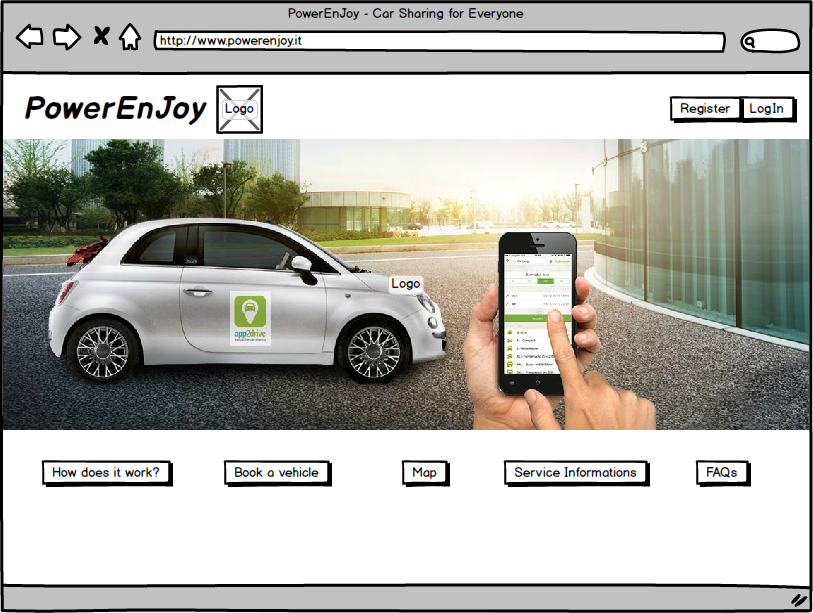
\includegraphics[scale=0.4]{img/webhome}
	\caption{PowerEnJoy website homepage}
\end{figure}
\FloatBarrier



\subsubsection{Security}

The system must ensure that all data is protected from unauthorized
access. Password should be saved on a DB hashed and salted.
Every input from the user and every request must be sanitized 
\iffalse
It must support communication protocols used by web applications and
devices on or within the network edge. These include network transport
protocols such as HTTP and SSL/TLS, plus proxy support.
\fi
\end{itemize}

\pagebreak{}




\subsubsection{Performance}


\subsubsection{Maintainability and Portability}




\subsubsection{Network connections}


\subsubsection{Cookies}



\subsubsection{Hardware requirement}
\todo[inline]{Matteo: da approfondire/inventare}
The communication between client and server is done using HTTPS REST API encrypted with TLS connections.
Nginx webserver and a large use of caching.
Google Maps API.



\subsubsection{Concurrent operations}

\pagebreak
\subsection{Use Case}

\subsubsection{User Registration}

\begin{center}
	
	\begin{tabular}{|l|>{\raggedright}p{10cm}|}
		\hline 
		Use Case Name & User Registration\tabularnewline
		\hline 
		\hline 
		Actors & Guest\tabularnewline
		\hline 
		Goal & {[}G1{]} Allow guests to register to ``PowerEnJoy'' service through both website or mobile application.\tabularnewline
		\hline 
		Preconditions & Guest hasn't registered to the webapp yet.\tabularnewline
		\hline 
		Postconditions & Guest is signed-up and promoted to ``PowerEnJoy'' User.\tabularnewline
		\hline 
		Normal Flow & \begin{enumerate}
			\item Guest accesses to the webapp or the mobile application
			\item Guest clicks on ``Sign Up'' button
			\item Guest fill Sign-up form fields, entering\\
			-Name\\
			-Surname\\
			-Email address\\
			-Password\\
			-Telephone Number\\
			-Driving License number
			\item Guest accepts the term of use
			\item Guest clicks on ``Confirm'' button\end{enumerate}
		\tabularnewline
		\hline 
		Exceptions & \begin{enumerate}
			\item At least one field is empty
			\item At least one field is invalid
			\item Entered email is already associated to another account\end{enumerate}
		\tabularnewline
		\hline 
	\end{tabular}
	\par\end{center}

\pagebreak
\subsubsection{User Login}
\begin{center}
	\begin{tabular}{|l|>{\raggedright}p{10cm}|}
		\hline 
		Use Case Name & User Login\tabularnewline
		\hline 
		\hline 
		Actors & User\tabularnewline
		\hline 
		Goal & {[}G2{]} Allow registered users to login and logout.\tabularnewline
		\hline 
		Preconditions & User has signed-up as PowerEnJoy User.\tabularnewline
		\hline 
		Postconditions & User is redirected to personal area.\tabularnewline
		\hline 
		Normal Flow & \begin{enumerate}
			\item User accesses to the webapp or the mobile application
			\item User clicks on ``Log-in' button
			\item User fills username and password fields of Log-in form
			\item User clicks on ``Submit'' button
			\end{enumerate}
		\tabularnewline
		\hline 
		Exceptions & \begin{enumerate}
		\item Invalid username and/or password
		\item At least one field is empty\end{enumerate}
		\tabularnewline
		\hline 
	\end{tabular}
	\par\end{center}

\begin{figure}[h]
	\centering
	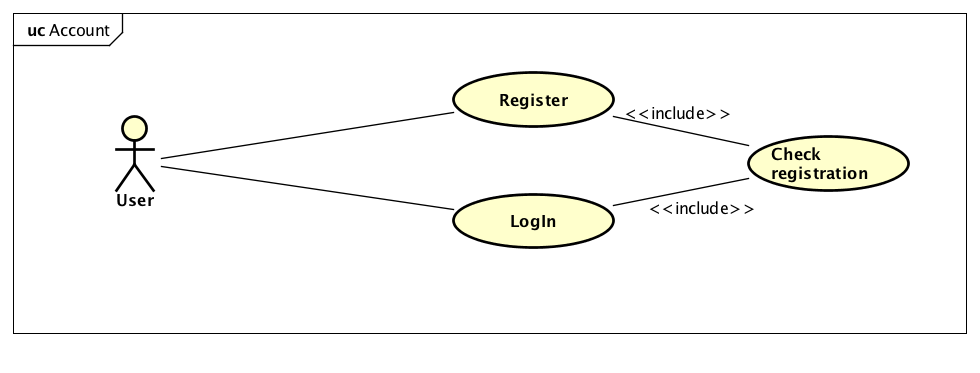
\includegraphics[scale=0.5]{img/usecase_login_registration}
	\caption{Use Case Login and Registration procedure. Refer to Goal 1 and 2}
\end{figure}
\FloatBarrier

\subsubsection{User Login}
\begin{center}
	\begin{tabular}{|l|>{\raggedright}p{10cm}|}
		\hline 
		Use Case Name & Personal information update\tabularnewline
		\hline 
		\hline 
		Actors & User\tabularnewline
		\hline 
		Goal & {[}G3{]} Allow authenticated users to modify their personal details and payment informations.\tabularnewline
		\hline 
		Preconditions & User has signed-up as PowerEnJoy User.\tabularnewline
		\hline 
		Postconditions & User's personal and payment information are updated with confirmation.\tabularnewline
		\hline 
		Normal Flow & \begin{enumerate}
			\item User accesses to the webapp or the mobile application
			\item User clicks on ``Log-in' button
			\item User fills username and password fields of Log-in form
			\item User clicks on ``Submit'' button
		\end{enumerate}
		\tabularnewline
		\hline 
		Exceptions & \begin{enumerate}
			\item Invalid username and/or password
			\item At least one field is empty\end{enumerate}
		\tabularnewline
		\hline 
	\end{tabular}
	\par\end{center}

